\chapter{Araztailea}\label{sec:webkontsola}

\section{Firefox-en Web Kontsola}

Webgune bat garatzean ezinbestekoa egingo zaigu programatutako kodea araztea eta zuzentzea. Horretarako, nabigatzaileak berak hainbat tresna laguntzaile eskaintzen dizkigu. Firefox-ek Web Kontsola\index{Web Kontsola} deritzona. Chrome-ren kasuan DevTools \index{DevTools}(\textit{Developer Tools}).

\begin{figure}[ht]
	\centering
\begin{tikzpicture}[framed]
\node[anchor=south west,inner sep=0] (image) at (0,0)
   {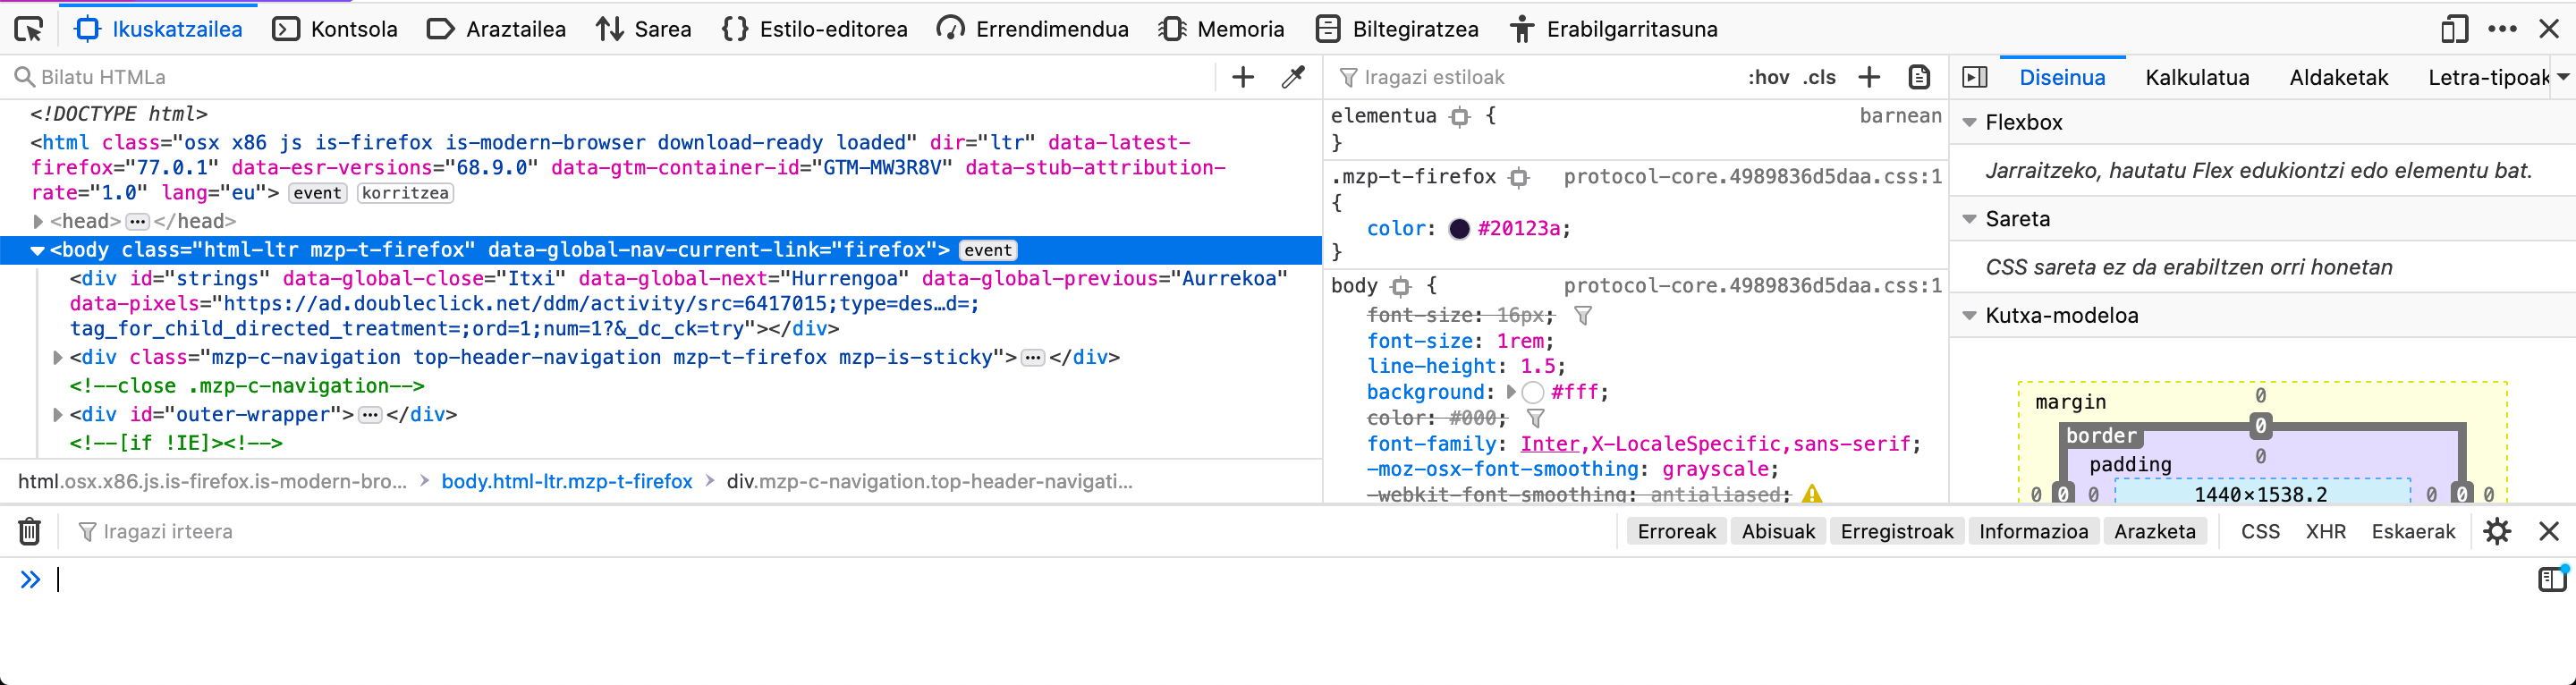
\includegraphics[trim=0cm 0cm 0cm 0cm, clip=true, width=1.0\textwidth]{img/webkontsola.png}};
\end{tikzpicture}
\caption{Firefox-en Web Kontsolak informazio andana eskainiko digu ikusten ari garen web orriaren inguruan.}
\label{fig:webkontsola}
\end{figure}

Kontsola irekitzeko, Firefox-en, \hl{Hobespenak / Web Garapena / Web Kontsola} hautatu. Bertan, hainbat fitxa aurkituko dugu. \hl{Ikuskatzailea}\index{Ikuskatzailea} izeneko erlaitza izango da goi-eskuineko aldean ikusiko dugun lehenengoa. Bertan sakatzean,  \ref{fig:webkontsola}. irudiko beheko 3 panelak ikusiko ditugu: uneko orriaren HTML kodea (bertan edozein nodo ezabatu edo aldatu dezakegu eta nabigatzailean berehala ikusi emaitza), unean hautatuta dugun HTML DOM zuhaitzen elementuaren CSS estiloak eta, eskuinaldean, elementu horri aplikatzen zaizkion ertzak eta marjinak, besteak beste. \hl{ESC} tekla sakatuz gero, kontsola irekiko da (beheko panela). Kontsolan gure JavaScript kodeen zirriborroak landu ditzakegu, eta uneko orrian kargatu diren scripten funtzioak eskuz exekutatu.

Behealdeko kontsolaren panela oso txikia iruditzen bazaigu, \hl{Kontsola} izeneko fitxan sakatu eta kontsola erabat irekiko da. 

Dena den, gure programatzaile-lanak batez ere \hl{Araztailea} (\textit{debugger})\index{debugger}\index{araztailea} izeneko fitxan izango dira. Web aplikazio profesionalak lantzeko, ezinbestekoa da araztailea ondo menderatzea. Hurrengo atalean araztailea nola erabiltzen den ikasiko dugu, adibide sinple batekin.

\section{Araztailea erabiltzen}

\begin{lstlisting}[language=HTML]
<html> <head> <title>Proba</title> <script src="proba.js"></script> </head>
<body>
  Araztailearekin lanean.
</body>
</html>
\end{lstlisting}


Demagun 3 puntuz osatutako arraya sortu dugula:

\begin{lstlisting}[language=JavaScript]
function Point(x,y){
  this.x = x;
  this.y = y;
}

let puntuak = [new Point(5,0), new Point(11,1), new Point(2,2)];

\end{lstlisting}

Jarraian, array horren puntu batzuk ezabatzeko agindua jasotzen dugu. Zehazki, x koordenatua 10 baino balio handiagoa dutenak. Otu ahal zaigun
lehenengo saiakera honako kodea izan daiteke. Baina ez da zuzena, zergatik?

\begin{lstlisting}[language=JavaScript]
let luzera = puntuak.length;
for(let i=0; i < luzera; i++){
    if (puntuak[i].x > 10)
        puntuak.splice(i,1);
}
\end{lstlisting}

Exekutatuz gero, \hl{if (puntuak[i].x > 10)} lerroan errore bat jasoko dugula ikusiko dugu (ikus \ref{fig:araztaile1}. irudia):

\begin{figure}[ht]
	\centering
\begin{tikzpicture}[framed]
\node[anchor=south west,inner sep=0] (image) at (0,0)
   {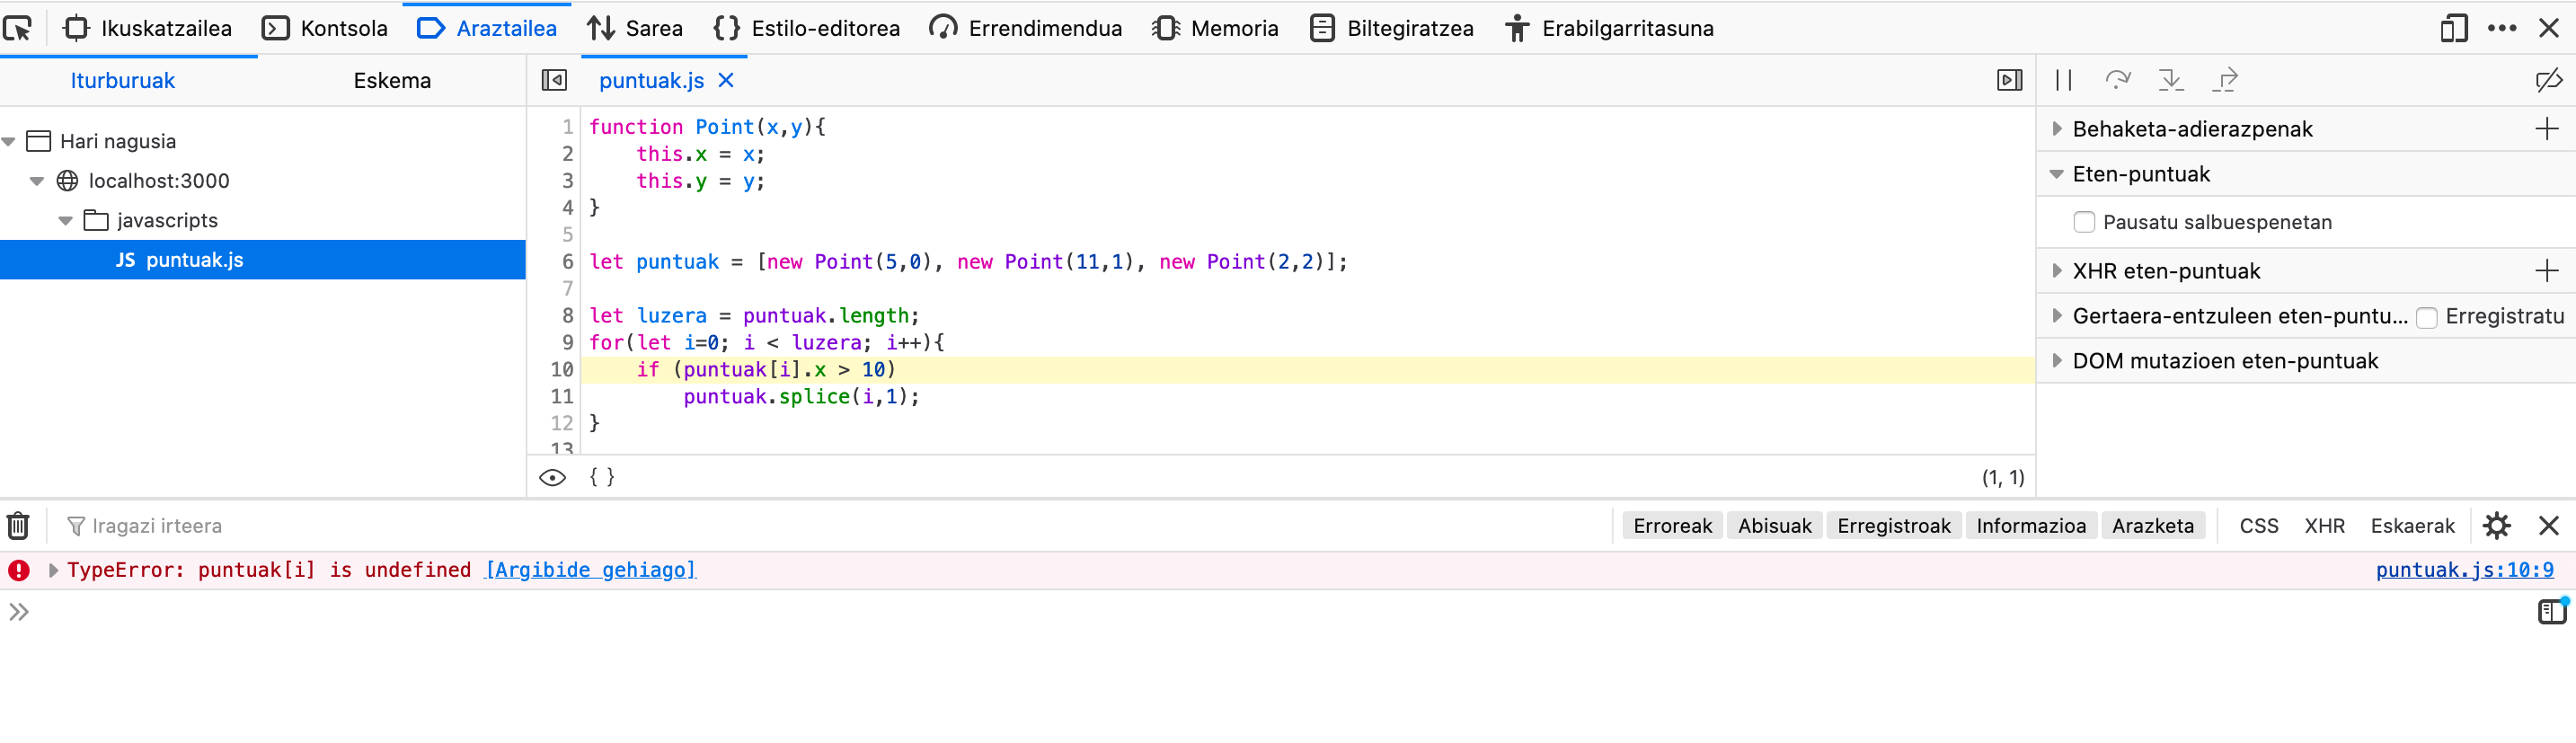
\includegraphics[trim=0cm 0cm 0cm 0cm, clip=true, width=1.0\textwidth]{img/araztaile1.png}};
\end{tikzpicture}
\caption{Araztailea nola erabiltzen den ikastea ezinbestekoa da taxuzko web aplikazio bat garatu nahi badugu.}
\label{fig:araztaile1}
\end{figure}

Eten-puntu\index{eten-puntu} bat (\textit{breakpoint}\index{breakpoint} bat) jarriko dugu lerro horretan jakin ahal izateko zer gertatu den. Hamargarren lerroan (lerro-zenbakiaren gainean) klik bat eginez, urdinez markatuko da eten-puntua.

\begin{figure}[ht]
	\centering
\begin{tikzpicture}[framed]
\node[anchor=south west,inner sep=0] (image) at (0,0)
   {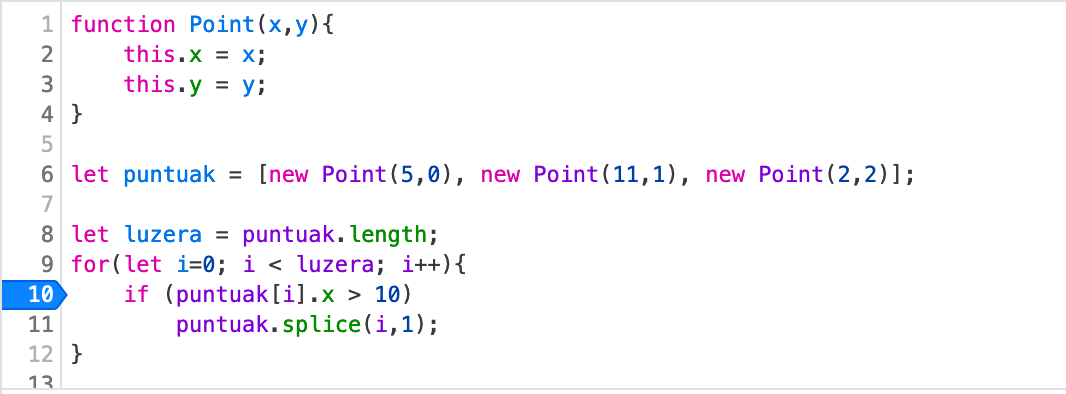
\includegraphics[trim=0cm 0cm 0cm 0cm, clip=true, width=1.0\textwidth]{img/araztaile2.png}};
\end{tikzpicture}
\caption{\textit{Breakpoint} edo eten-puntuak lerro-zenbakiaren gainean klik eginez zehaztuko ditugu.}
\label{fig:araztaile2}
\end{figure}

Orain orria berriro kargatzean, kodea martxan jarri eta eten-punturaino helduko da, bertan exekuzioa etenez. Araztailearen panelak ere irekiko dira. Eskuinaldeko panelean, behaketa-adierazpenak azpiatalaren barruan, \hl{+}  botoian sakatu eta \hl{i} aldagaiaren balioa ikusi nahi dugula adieraziko dugu. Baita \hl{luzera} eta \hl{puntuak} arrayaren edukia ere (ikus \ref{fig:araztaile3}. irudia).

\begin{figure}[ht]
	\centering
\begin{tikzpicture}[framed]
\node[anchor=south west,inner sep=0] (image) at (0,0)
   {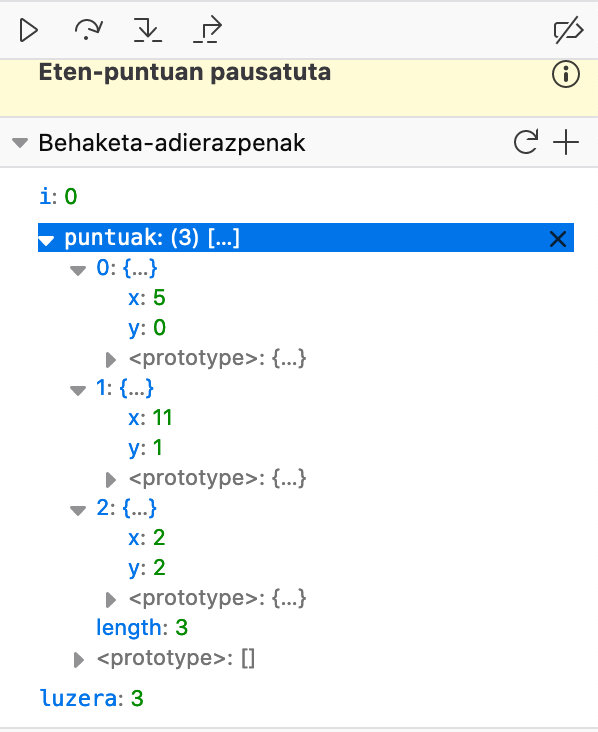
\includegraphics[trim=0cm 0cm 0cm 0cm, clip=true, width=0.5\textwidth]{img/araztaile3.png}};
\end{tikzpicture}
\caption{Programa pausoz pauso egikaritzean, aldagaien balio guztiak monitorizatu ahal ditugu \textit{debugger}-aren behaketa-adierazpenak\index{behaketa-adierazpen} atalean.}
\label{fig:araztaile3}
\end{figure}

Ohart zaitez \hl{i} aldagaiaren balioa, eten-puntuan, une honetan 0 dela. \hl{Luzera}, 3. Eta, beraz, arraya zeharkatzen hasi gara, oraindik ez dugu ezer ezabatu bertatik.

Exekuzioa etenda dago. Hurrengo lerroarekin jarraitzeko, pauso bat aurrera egin behar dugu, alegia, \ref{fig:araztaile4}. irudiko 2. gezian sakatu (edo Ctrl+F10). Botoi horri ingelesez ``\textit{Step into}'' deritzo \index{step-into}.

\begin{figure}[ht]
	\centering
\begin{tikzpicture}[framed]
\node[anchor=south west,inner sep=0] (image) at (0,0)
   {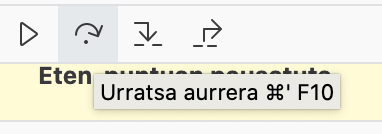
\includegraphics[trim=0cm 0cm 0cm 0cm, clip=true, width=0.5\textwidth]{img/araztaile4.png}};
\end{tikzpicture}
\caption{F10 tekla sakatzean urrats bat aurrera egingo dugu gure kodean. F8 (\textit{Play}) tekla sakatuz exekuzioa aurrera egingo du hurrengo eten-puntua aurkitu arte.}
\label{fig:araztaile4}
\end{figure}

Baldintza betetzen ez denez (\hl{puntuak[0].x = 5} da), ez gara 11. lerroan sartuko eta zuzenean \textit{for} begiztara egingo dugu jauzi. Ctrl+F10 sakatu berriro eta \hl{i} aldagaiaren balioa unitate batean gehituko da (i=1). Orain (Ctrl+F10 berriro), \textit{for} begiztaren baldintza aztertuko da ( \hl{i < luzera} ) eta betetzen denez, hurrengo pausoan berriro \textit{if} baldintzan sartuko gara. Orain baldintza beteko da (\hl{puntuak[1].x = 11}) eta, beraz, \hl{puntuak.splice(1,1)} exekutatuko da. Horrek \hl{puntuak} arrayari elementu bat kenduko dio. 


\begin{figure}[ht]
	\centering
\begin{tikzpicture}[framed]
\node[anchor=south west,inner sep=0] (image) at (0,0)
   {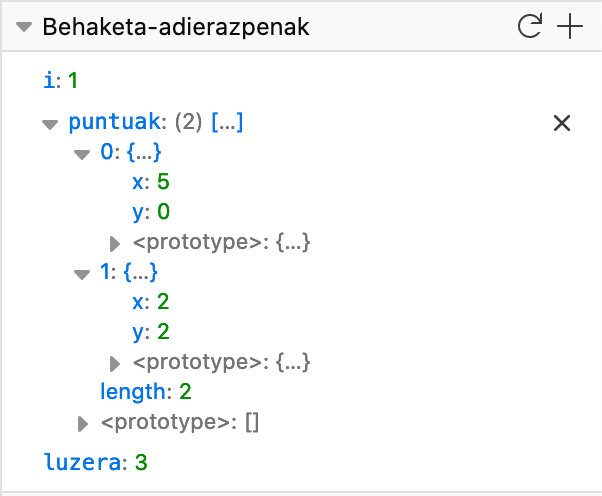
\includegraphics[trim=0cm 0cm 0cm 0cm, clip=true, width=0.5\textwidth]{img/araztaile5.png}};
\end{tikzpicture}
\caption{Array baten edukia behaketa-adierazpenekin oso modu erosoan ikusi ahalko dugu.}
\label{fig:araztaile5}
\end{figure}

Baina adi, \hl{luzera} aldagaiaren balioa ez da eguneratzen! Ikus \ref{fig:araztaile5}. irudia. Hots, arrayan hasieran baino elementu bat gutxiago badugu ere, \hl{luzera} aldagaia ez da aldatu. Hurrengo exekuzio-lerroan, \hl{i++} egin eta \hl{i=2} bilakatuko da. Arrayak soilik 2 elementu ditu, beraz, \hl{if (puntuak[2].x = 0)} aztertzean, errore bat jasoko dugu (\hl{puntuak[2]} elementua ez baita existitzen!).

Konpontzeko, agian beste soluzio hau otu ahal zaigu:

\begin{lstlisting}[language=JavaScript]
let puntuak = [new Point(5,0), new Point(11,1), new Point(2,2)];
for(let i=0; i < puntuak.length; i++){
    if (puntuak[i].x > 10)
        puntuak.splice(i,1);
}
\end{lstlisting}

Adibidean emandako puntuekin ondo doa, baina ez da soluzio zuzena ere. Zergatik? Puntu berri bat txertatuz gero:

\begin{lstlisting}[language=JavaScript,numbers=none]
let puntuak = [new Point(5,0), new Point(11,1),  new Point(15,1), new Point(2,2)];
\end{lstlisting}

eta \textit{debugger}-arekin pausoz pauso exekutatuz gero, hau ikusiko dugu:

\begin{figure}[ht]
	\centering
\begin{tikzpicture}[framed]
\node[anchor=south west,inner sep=0] (image) at (0,0)
   {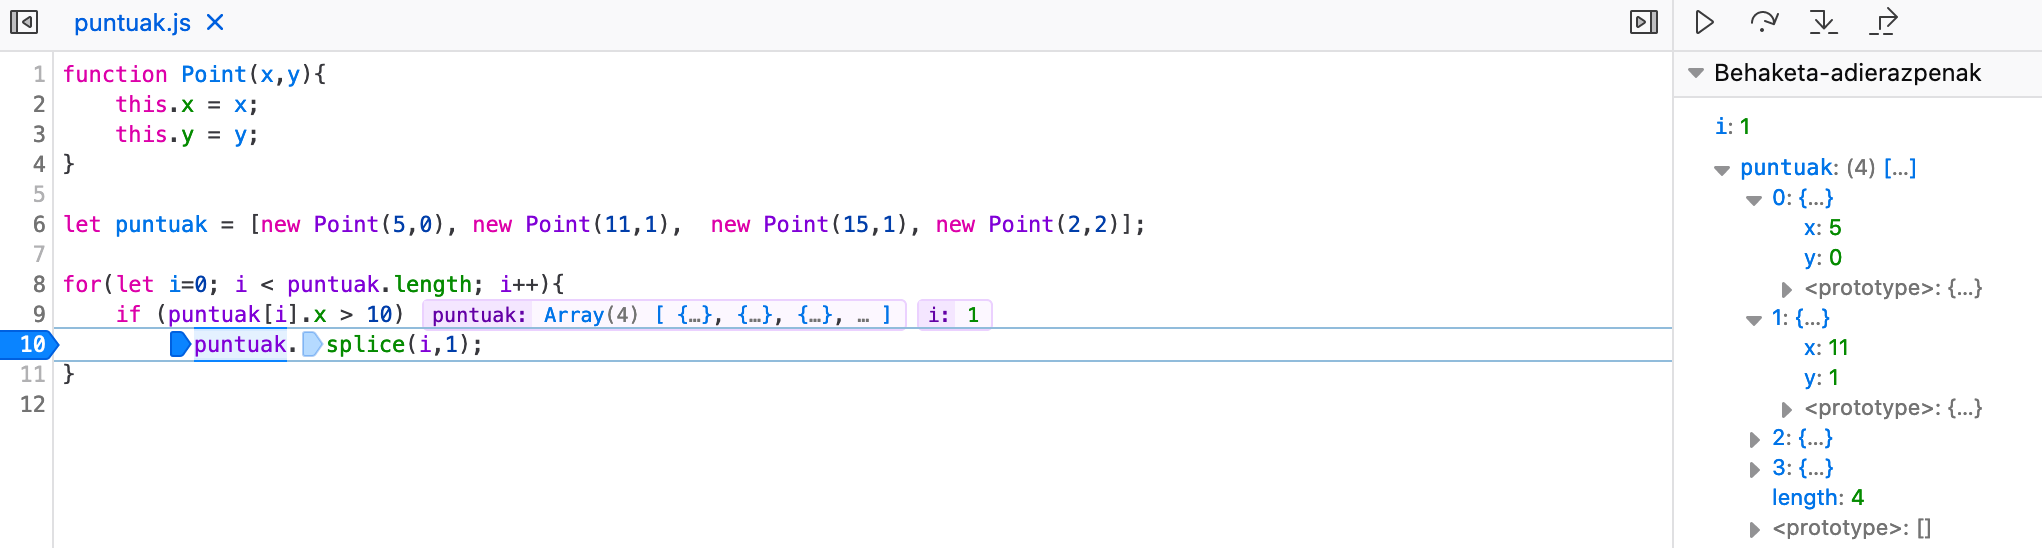
\includegraphics[trim=0cm 0cm 0cm 0cm, clip=true, width=1.0\textwidth]{img/araztaile6.png}};
\end{tikzpicture}
\caption{Exekuzioa urratsez urrats zeharkatzean, araztaileak lerro bakoitzaren ondoan bertan aldatu diren aldagaien balioak adieraziko ditu, kodearen ondoan —ikus 9. lerroaren eskuinaldea—.}
\label{fig:araztaile6} 
\end{figure}

 \hl{i=1} denean, \hl{puntuak[1]} ezabatu egingo dugu. Une honetan arrayaren edukia hau da:
 
 \begin{lstlisting}[language=JavaScript,numbers=none]
 [Point(5,0), Point(15,1)]
 \end{lstlisting}

Hurrengo iterazioan \hl{i++} egitean, \hl{i=2} bilakatuko da eta \textit{for} begiztatik irten egingo gara, azkenengo puntua (15,1) tratatu gabe!

Egoera zuzentzea ez da zaila: arraya lehenengo elementutik aztertzen hasi ordez, azkenengo elementutik lehenengo elementura zeharkatuko dugu.

\begin{lstlisting}[language=JavaScript,numbers=none]
for (let i=puntuak.length-1; i>=0; i--){
  if (puntuak[i].x > 10)
     puntuak.splice(i,1);
}
\end{lstlisting}

Gogoan izan ariketa ez zela arazoa konpontzea, baizik eta araztailea erabiltzen ikastea arazoaren arrazoia aurkitzeko.

\subsection{Baldintzazko eten-puntuak}

Demagun gure arrayan sei puntu sortu ditugula. Laugarren puntuan gaudenean kodearen portaera aztertu nahi dugu. Baina horraino heltzeko, pausoz pauso exekutatzea, prozedura neketsu eta traketsa bilaka daiteke (F10 hainbat aldiz sakatu beharko dugu... eta 4. posizioan egon ezean, 400. posizioan egonez gero, prozedura ezinezkoa litzakete). Zer egin? Kasu hauetan baldintzazko eten-puntuak oso baliagarriak bilakatuko zaizkigu. Alegia, eten-puntuek kodearen exekuzioa geratuko dute, soilik ezarritako baldintza betetzen denean. Horretarako, eten-puntuak ezarri, haien gainean eskuineko botoia sakatu eta \hl{Editatu baldintza} hautatu. Eten-puntuak orain laranjaz marraztuko dira eta eskuinaldean, eten-puntuen panelean, ezarritako baldintza agertuko da (kasu honetan \hl{i==3}, ikus \ref{fig:araztaile7}. irudia).

\begin{figure}[ht]
	\centering
\begin{tikzpicture}[framed]
\node[anchor=south west,inner sep=0] (image) at (0,0)
   {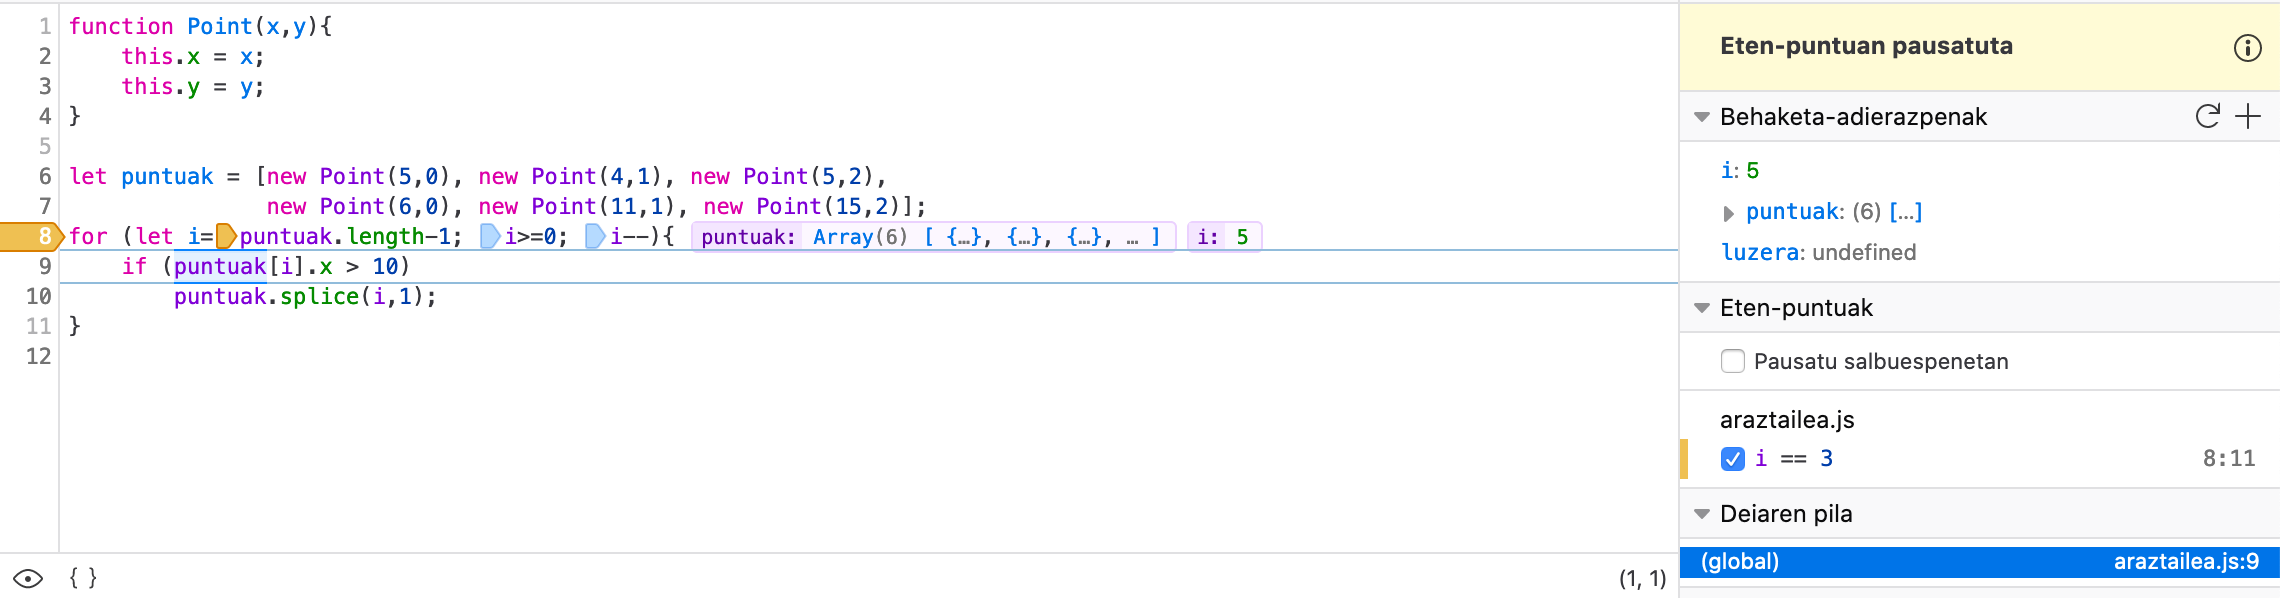
\includegraphics[trim=0cm 0cm 0cm 0cm, clip=true, width=1.0\textwidth]{img/baldintzazkoetenpuntuak.png}};
\end{tikzpicture}
\caption{Baldintzazko eten-puntuak ezarri ondoren, \faPlay \, botoian sakatu eta kodearen exekuzioa baldintza bete arte exekutatuko da, puntu horretan etenez.}
\label{fig:araztaile7} 
\end{figure}

Bukatzeko \faPlay \index{Play} ikurrean (edo F8 teklan) sakatu. Exekuzioak aurrera egingo du \hl{i==3} baldintza bete arte.

\begin{lstlisting}[language=JavaScript]
let puntuak = [new Point(5,0), new Point(4,1), new Point(5,2), new Point(6,0), new Point(11,1), new Point(15,2)];
for (let i=puntuak.length-1; i>=0; i--){
    if (puntuak[i].x > 10)
        puntuak.splice(i,1);
}
\end{lstlisting}